\documentclass[
    convert={density=300,outext=.png}
]{standalone}
\usepackage{graphicx}

\usepackage{tikz}

\usetikzlibrary{arrows,decorations.pathreplacing,backgrounds,positioning,fit}

\begin{document}
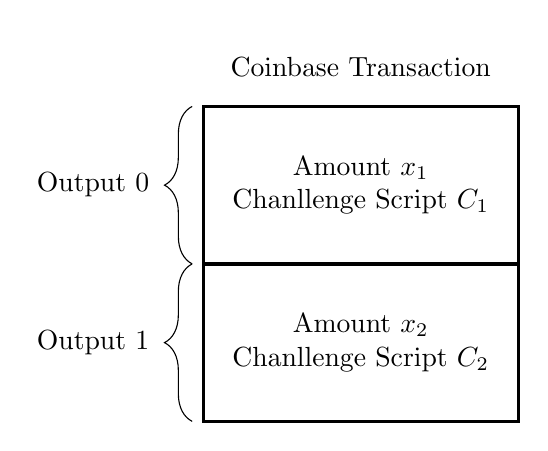
\begin{tikzpicture}
    [
        Field/.style={rectangle,minimum width=4cm,minimum height=2cm,draw,very thick, align=center},
        TextBox/.style={minimum width=4cm, minimum height=1cm, align=center}
    ]
    \node[TextBox] (Coinbase) at (2,4.5) {Coinbase Transaction};
    \node[Field] (Output0) at (2,3) {
        Amount $x_1$\\ Chanllenge Script $C_1$};
    \node[Field] (Output1) at (2,1) {Amount $x_2$ \\ Chanllenge Script $C_2$};

    \draw[decorate,decoration={brace,amplitude=10pt,raise=4pt},yshift=0pt] (0,2) -- (0,4)
        node [black,midway,xshift=-1.4cm] {Output 0};
    \draw [decorate,decoration={brace,amplitude=10pt,raise=4pt},yshift=0pt] (0,0) -- (0,2)
        node [black,midway,xshift=-1.4cm] {Output 1};
\end{tikzpicture}

\end{document}